\chapter{Revisão Sistemática}\label{cap_trabalho_academico}
O termo Revisão Sistemática (RS) é utilizado para se referir a uma metodologia específica de pesquisa, desenvolvida a fim de identificar, avaliar e interpretar as evidencias disponíveis relevantes para um determinado tema, ou questão de pesquisa, ou área de tópico, ou fenômeno de interesse \cite{biolchini2005, kitchenham2004}. A perspectiva conceitual mais ampla propõe uma abordagem definida em três fases principais, sendo estas, o planejamento da revisão, a condução da revisão e a apresentação dos resultados da revisão \cite{biolchini2005}. 

O planejamento da revisão define a identificação do que é necessário para a revisão e o desenvolvimento do protocolo que a direciona. A condução da revisão identifica a pesquisa, a seleção dos estudos primários, a avaliação da qualidade dos estudos, a extração e a síntese dos dados. E por fim a apresentação da revisão é a documentação de todo o trabalho executado \cite{kitchenham2004}.

Neste capitulo estão descritos os métodos e os resultados extraídos da revisão sistemática sobre sistemas de apoio a decisão para nutrição hospitalar, suas principais funcionalidades, características e metodologias utilizadas.

\section{Planejamento da Revisão}

Na fase de planejamento, baseando-se em \citeonline{biolchini2005}, foi construída a formularização das perguntas da pesquisa onde foram definidos o objetivo: analisar dados estratégicos sobre nutrição clínica em hospitais, e as características de qualidade e amplitude da pergunta, as quais são apresentadas no \autoref{quadro_formularizacaoPergunta}.
\newline
\newline
\newline

\begin{quadro}[htb]
\caption{\label{quadro_formularizacaoPergunta}Formularização das questões.}
\label{}
\begin{tabular}{|p{3cm}|p{8cm}|}
	\hline
	\textbf{Problema}       & Entender a disponibilização de dados sobre o ambiente nutricional clinico-hospitalar no Brasil e no mundo e a qualidade dos dados disponibilizados para tomadas de decisões eficientes.  \\ \hline
	\textbf{Palavras-chave} & Gerenciamento, Análise, Dados, Acompanhamento, Nutricional, Hospital, \textit{KPI}, Tomada de decisão , Apoio a decisão.   \\ \hline
	\textbf{Intervenção}    & Utilização de análise de dados e plataformas de \textit{Business Intelligence} em Hospitais e seus departamentos de Nutrição Clínica.   \\ \hline
	\textbf{Controle}       & Planilhas de 2019 das triagens realizadas pela unidade de nutrição clínica do HU/UFS.
 \\ \hline
	\textbf{Efeito}         & Referências de \textit{KPI}’s utilizadas em estudos anteriores e/ou projetos de \textit{Business Intelligence} focados na área da nutrição. \\ \hline
	\textbf{População}      & Redes hospitalares. \\ \hline
	\textbf{Aplicação}      & Gestores de hospitais e departamentos de nutrição, nutrólogos, analistas de B.I.\\ \hline
\end{tabular}
\fonte{Autor.}
\end{quadro}

Com os requisitos de formularização da pesquisa definidos foram criadas as seguintes questões de pesquisa:

µ1: Como as pesquisas tratam o gerenciamento e a análise dos dados clínicos sobre o acompanhamento nutricional dos pacientes nos hospitais?

µ2: Como os hospitais extraem Indicadores-chave de desempenho (KPI’s) para análise de dados de acompanhamento nutricional?

µ3: De que forma esses dados são utilizados e impactam nas tomadas de decisão dos setores de gestão e assistenciais dos estabelecimentos hospitalares?


\section{Condução da Revisão}

Na fase de condução, foram definidas as fontes onde foram realizadas as buscas dos estudos primários, e após definidos os critérios de inclusão e exclusão dos estudos foi realizado o procedimento de seleção \cite{biolchini2005}. 


\subsection{Seleção das fontes}

A etapa foi realizada pelo método de pesquisa em motores de busca na web. Nesta fase foram escolhidas 6 bases bibliográficas, nas quais foram realizadas as buscas para os trabalhos selecionados. Esta atividade foi realizada no mês de dezembro de 2020 e os resultados retornados correspondem ao conteúdo disponível até esta data. As bases escolhidas foram as seguintes:
\begin{itemize}
 \item ACM Digital Library\footnote{ACM Digital Library: \url{https://dl.acm.org}};
 \item IEEE Xplorer\footnote{IEEE Xplorer: \url{https://ieeexplore.ieee.org/Xplore/home.jsp}};
 \item MEDLINE (Pubmed)\footnote{MEDLINE (Pubmed): \url{https://pubmed.ncbi.nlm.nih.gov}};
 \item Scopus (Elsevier)\footnote{Scopus (Elsevier): \url{https://www.scopus.com/home.uri}};
 \item Springer Link\footnote{Springer Link: \url{https://link.springer.com}};
 \item ScienceDirect\footnote{ScienceDirect: \url{https://www.sciencedirect.com}}.
\end{itemize}

Por meio das palavras-chave descritas no \autoref{quadro_formularizacaoPergunta} foram criadas as strings de busca utilizadas na bases bibliográficas, conforme \autoref{quadro_stringsDeBusca}. O uso dos termos \textit{Business Intelligence}, \textit{Business Analytics} e \textit{Decision Support System} foram considerados por não haver, segundo (\textbf{TURBAN}) uma definição concreta na literatura e por serem comumente atribuídos como termos guarda-chuva à sistemas de apoio a decisão. 

\begin{quadro}[htb]
\caption{\label{quadro_stringsDeBusca}\textit{Strings} de busca.}
\label{}
\begin{tabular}{|p{2cm}|p{9cm}|}
	\hline
	\textbf{String 01}	& \textit{"business intelligence" AND "hospital nutrition"}.  \\ \hline
	\textbf{String 02}	& \textit{"business intelligence" AND "clinical nutrition"}.   \\ \hline
	\textbf{String 03}	& \textit{"business intelligence" AND nutrition}.   \\ \hline
	\textbf{String 04}	& \textit{"business analytics" AND "hospital nutrition"}.	\\ \hline
	\textbf{String 05}	& \textit{"business analytics" AND "clinical nutrition"}. \\ \hline
	\textbf{String 06}	& \textit{"business analytics" AND nutrition}. \\ \hline
	\textbf{String 07}	& \textit{"decision support system" AND "hospital nutrition"}.\\ \hline
    \textbf{String 08}	& \textit{"decision support system" AND "clinical nutrition"}.\\ \hline
    \textbf{String 09}	& \textit{"decision support system" AND "clinical nutrition"}.\\ \hline
\end{tabular}
\fonte{Autor.}
\end{quadro}

Os resultados retornados por cada \textit{string} de busca foram somados a um único montante de artigos, os quais passaram pelas etapas seguintes de seleção dos estudos. 

\subsection{Seleção dos estudos}
Esta etapa apresenta os critérios pelos quais os estudos foram avaliados. Existe a necessidade de se definir tais critérios porque uma busca realizada em mecanismos da web acabam por retornar um grande número de artigos que não correspondem à pergunta de pesquisa, devido ao fato de algumas palavras-chave possuírem significados diferentes ou serem utilizadas em estudos que não tratam do tema da pesquisa de revisão sistemática \cite{biolchini2005, kitchenham2004}.

De acordo com as questões de pesquisa e com o objetivo da revisão foram definidos
Critérios de Inclusão e Exclusão para o tema da pesquisa com o objetivo de nortear a seleção dos artigos na fase de condução da revisão, como apresentados abaixo.

Os critérios de inclusão (CI) considerados na seleção dos artigos foram:
\begin{itemize}
    \item \textbf{CI1}. O artigo apresenta ferramentas de \textit{Business Intelligence};
    \item \textbf{CI2}. O artigo apresenta ferramentas de análise e apoio à decisão;
    \item \textbf{CI3}. O artigo conter produto com funcionalidades relacionadas ao apoio à decisão;
    \item \textbf{CI4}. O artigo aborda sobre impactos positivos no uso/implantação de ferramentas de apoio a decisão;
    \item \textbf{CI5}. O artigo aborda sobre impactos negativos no uso/implantação de ferramentas de apoio a decisão;
    \item \textbf{CI6}. O artigo contém indicadores de performance (\textit{Key Performance Indicator}).
\end{itemize}

Os critérios de exclusão (CE) considerados na seleção dos artigos foram:
\begin{itemize}
    \item \textbf{CE1}. O artigo não deve ser incompleto ou apenas resumo;
    \item \textbf{CE2}. O estudo não deve ser capítulo de livro;
    \item \textbf{CE3}. O artigo não está disponível para download em seu formato completo na web;
    \item \textbf{CE4}. Artigos duplicados devido às varias bases bibliográficas e múltiplas  strings de busca;
    \item \textbf{CE4}. O artigo não pode ser anterior ao ano de 2010;
\end{itemize}


\subsection{Procedimentos de seleção}

Após realizada a busca inicial nas bases de pesquisa, 4.727 estudos foram encontrados. Por possuírem a função de indexadores de conteúdo o \textit{ScienceDirect} e o \textit{SpringerLink} foram as bases que mais retornaram resultados, com 2.248 e 1.835 estudos respectivamente como mostra a \autoref{fig_graficoSelecaoInicialEstudos} a seguir.
\newline
\newline

\begin{figure}[htb]
	\caption{\label{fig_graficoSelecaoInicialEstudos}Gráfico de seleção inicial de estudos por bases bibliográficas.}
	\begin{center}
	    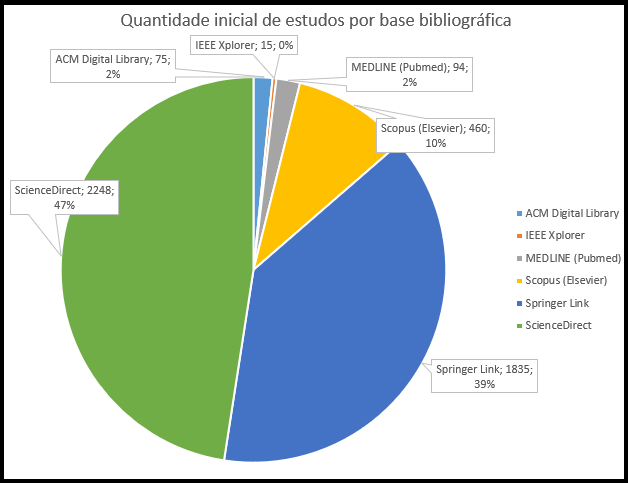
\includegraphics[scale=0.5]{Imagens/grafico - selecao inicial de estudos por base.png}
	\end{center}
	\legend{Fonte: Autor.}
\end{figure}

Porém o termo \textit{nutrition} resultou em uma grande quantidade de estudos relacionados à técnicas de nutrição animal e medições de nutrientes vegetais, que não são relevantes para este trabalho. Estes resultados foram avaliados por seus resumos na etapa de inclusão e 2.625 estudos não foram incluídos para avaliações mais significativas. É possível conferir o comparativo de resultados por strings de busca na \autoref{fig_graficoSelecaoInicialEstudosStrings}.

\begin{figure}[htb]
	\caption{\label{fig_graficoSelecaoInicialEstudosStrings}Gráfico de seleção inicial de estudos por \textit{strings} de busca.}
	\begin{center}
	    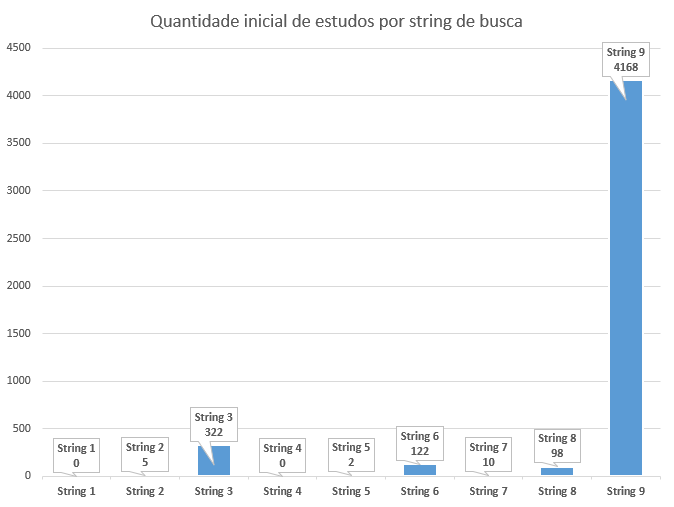
\includegraphics[scale=0.52]{Imagens/grafico - selecao inicial de estudos por string.png}
	\end{center}
	\legend{Fonte: Autor.}
\end{figure}

Após a execução da busca inicial de estudos, na etapa seguinte após análise de títulos e resumos, 54 resultados satisfizeram ao menos um dos critérios de inclusão e foram selecionados como estudos primários, como mostra a \autoref{fig_graficoProcessoInclusaoExclusaoArtigos}. 

Na etapa de exclusão, mostrada na \autoref{fig_graficoProcessoInclusaoExclusaoArtigos}, os artigos que foram coincidentes com ao menos um dos critérios de exclusão foram removidos da revisão. Do total de estudos primários 26 resultados foram retirados por estarem duplicados, 11 estudos foram removidos por não tratarem do tema abordado neste trabalho e 17 artigos foram selecionados,\textbf{ CONFORME QUADRO } para a etapa de extração dos dados, e assim, responder as questões da pesquisa definidas nesta revisão.  
- 

\section{Analise dos resultados}
texto texto texto texto texto texto texto texto texto texto texto texto texto texto texto texto texto texto texto texto texto texto texto texto texto texto texto texto texto texto texto texto texto texto texto texto texto texto texto texto texto texto texto texto texto texto texto texto texto texto texto texto texto texto texto texto texto texto texto texto texto texto texto texto texto texto texto texto texto texto texto texto texto texto texto texto texto texto texto texto texto texto texto texto texto texto texto texto texto texto texto texto texto texto texto texto texto texto texto texto texto texto texto texto texto texto texto texto texto texto texto texto texto texto texto texto texto texto texto texto texto texto texto texto texto texto texto texto texto texto texto texto texto texto texto texto texto texto texto texto texto texto texto texto texto texto texto texto texto texto texto texto 